
 \begin{figure}
	\centering
	\scalebox{0.80}{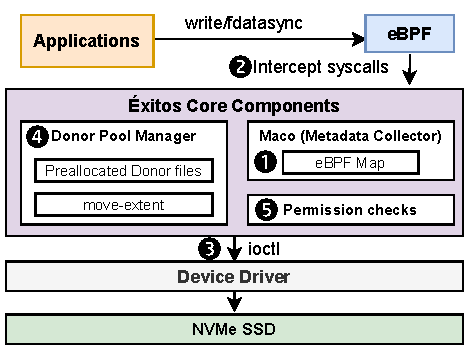
\includegraphics[width=\linewidth]{fig/design/structure.pdf}}
	%	\vspace{0ex}	
	\caption{The Architecture of \odes.}	\label{fig:architecture} %TODO: redraw -- wangc@2026.09.09-18:52
	\vspace{-3ex}
\end{figure}

\section{The Design of \odes}\label{sec:design}

\subsection{An Overview of \odes}\label{sec:design:overview}

%Many applications rely on file writes to store data. 
%Examples include logging data for databases and saving results produced in scientific computing.
\odes is specifically designed to build a %new, sound, and
 fast  shortcut I/O path for database logging.
It is an {\em all-in-software} solution aiming to reduce the heavy software tax charged on logging writes.
%% It aims 
%In order 
%%to minimize the heavy software tax 
%%%charged on database logging writes. % in these scenarios,
\odes %. To do so, it 
  separates management actions from actual I/O delivery.
%associated with file writes. 
 As depicted by the architecture of \odes shown in \autoref{fig:architecture}, it intercepts file write and fdatasync for database logging 
 using the eBPF hooks. 
The  intercepted operations are then redirected via ioctl interfaces %~\cite{ioctlWik84:online} 
and   delivered to the device driver (Section \ref{sec:design:components}).



\odes is applicable to both preallocated and   growing log files. 
For preallocated ones, \odes extracts  per-file offset-to-block mappings at initialization and manages these metadata using an in-memory \emph{Metadata Collector} (Maco) structure. 
For  a non-preallocated  log, \odes employs a {\em donor-based preallocation-like strategy} that pre-reserves 
contiguous  block ranges and exploits Ext4's \textit{move-extent} feature~\cite{ext4moveextent} to 
efficiently extend file space  with minimized 
runtime cost (Section \ref{sec:design:donor}). 
This   enables \odes to handle a growing log file in its fast path.
%a growing log file to be operable in \odes's  fast shortcut path.

Furthermore,
to make 
%
 %\odes is 
   an effectual and self-contained design, we optimize \odes in the dimensions of
 %It is
% optimized for 
 scalability, comprehensiveness, and compatibility (Section \ref{sec:design:discussion}). 

The primary technical novelty of \odes lies in two points. First, \odes builds its
shortcut I/O path on per-file mappings that stay stable: once a database log file
has been preallocated, the file's mappings from in-file offsets to device block
numbers remain unchanged throughout the period in which the log file stays open.
Stable per-file mappings make an all-in-software shortcut both feasible and safe,
because the block numbers that \odes issues I/Os to are the ones that Ext4 itself
has computed. Second, \odes turns move-extent from a feature for defragmentation
into a means of supplying space online, so that per-file mappings stay equally
stable for a growing log file.

%scalable with per-core distributed structures. It provides different levels of permission  checks. It is also compatible with various storage devices.
%In summary, it 
% a self-contained design with
%scalability with multi-core CPU,
% comprehensive access permission checks,
% and compatibility with various storage devices.


\iffalse
\begin{comment}
Besides databases,
  applications that rely on persistent file writes to  store data, can benefit
from the 
%\odes provides an
   %efficient and secure 
 shortcut \odes provides %with high efficiency
 %for applications that rely on file writes, especially persistent stores, to save data 
 (Section \ref{sec:design:discussion}).
\end{comment}
\odes takes advantage of file system's space management and access controls while
leveraging the latest eBPF, ioctl, and io\_uring techniques.
% significantly optimizing write performance.
%(see Section \ref{sec:design:security}).
More importantly, it manages to bypass most software layers and largely reduces the runtime tax (Section~\ref{sec:design:summary}). 
\fi



\subsection{The Shortcut of \odes}\label{sec:design:components}


Let us take a preallocated log file to 
%We firstly %focus on handling writes efficiently for preallocated files.
%Let us firstly 
illustrate the core functionality of \odes.
%how \odes efficiently handles file write and fdatasync issued to it. %a preallocated file.
% As for files that gradually grow for expansion, we will introduce a preallocation-like strategy  in Section \ref{sec:design:donor}.
%In practical, one
 One such file  has a stable structure, 
%virtually undergoing no space
%
%a log file, once preallocated and initialized,
%to a preallocated file,  
% undergoes  virtually no change in its structural layout, without 
without any space reallocation or alternation of access permission.
%undergoes no space reallocation or alternation of access permission,
%so it
%A  file, once preallocated and initialized, 
Particularly, it has
%all device blocks of the file remain stable. 
%The stable structural layout means 
fixed per-file mappings from
 in-file offsets to device block numbers. 
% 
 %TODO: what does modern file systems like Ext4 handle deletion (truncation) of a few middle blocks? -- wangc@2025.09.09-19:21

 %a prealloaction-like strategy to handle the files write .
%has a stable structural layout.

\textbf{Workflow.} \autoref{fig:architecture} decomposes \odes's main components
and the workflow that \odes follows to handle a persistent write for database logging.
It firstly initializes the in-memory Maco structure for the log file (\ding{202} in \autoref{fig:architecture}).
At runtime,  \odes intercepts file write and fdatasync syscalls
(\ding{203}) and proceeds them in its own shortcut path (\ding{204}).
Next we would detail these three steps.

\textbf{Metadata management.}
As mentioned, % in Section \ref{sec:motivation},
it is essential but time-consuming for a logging write
to locate device blocks   by querying the log file's extent tree.
% for mapping information. %  is critical and time-consuming. %in  locating .
 \odes duplicates  the mappings of a preallocated file in its Maco structure for quick reference. 
\autoref{fig:prepare} describes an example that a log file receives
three contiguous block ranges after preallocation. % are preallocated to a log file.
 At initialization, i.e., when opening the log   file, \odes extracts  mappings from the file's extent tree
between  in-file offsets (e.g., 4096 and 8192 in   \autoref{fig:prepare}) and    block numbers (resp. 3608 and 5444). 
\odes neatly reorganizes this metadata
%This metadata is neatly reorganized
 within an in-memory eBPF map that stores the file descriptor, in-file offsets, base block numbers and lengths for block ranges, thereby enabling prompt block-level addressing. %%%%, essential for optimizing WAL operations simulated using fio. 
%By collecting this metadata with a ,  
%Preallocation helps to fix and retrieve this mapping metadata in advance. 
At runtime,
regarding block numbers found in the Maco structure,
\odes   %  accordingly
redirects   write and fdatasync requests to the device driver. % with correct block numbers.
%when the LBAs are known.




% \textbf{Runtime interception.} To intercept file operations,
% \odes employs {\em syscall tracepoints} that are static kernel instrumentation points characterized by minimal runtime overhead. 
% Tracepoints avoid the cost of dynamic instrumentation, making them ideal for latency-sensitive   operations~\cite{TracingL22:online}.
% %TheeBPFR54:online,
% \odes loads and runs these interception programs with bpftime~\cite{bpftime}, an
% eBPF runtime that is compatible with the standard eBPF toolchain.
% \odes obtains a list of log files from a configuration file that the database
% already reads, and \odes intercepts only the write and fdatasync requests issued to
% the log files on the list. Requests issued to any other file keep taking the
% conventional path, so a database needs no change to the source code of the
% database. Before issuing an ioctl request, \odes checks that the in-file
% offset and the length of the request fall inside one of the block ranges that the
% Maco structure has registered for the file descriptor in question. A request whose
% in-file offset and length fall outside every registered block range returns to the
% conventional path for handling instead of entering the shortcut I/O path of \odes.

\textbf{Runtime interception.}
\odes intercepts file operations using syscall tracepoints, which provide
low-overhead static kernel instrumentation suitable for latency-sensitive
paths~\cite{TracingL22:online}. The interception programs are executed by
bpftime~\cite{bpftime}.
\odes obtains a list of log files from a configuration file already used by
the database and intercepts only \texttt{write} and \texttt{fdatasync} requests
to the listed log files. All other requests continue through the conventional
I/O path. This design requires no changes to the database source code. Before
entering the shortcut path, \odes verifies that the request falls within a
block range registered in the Maco structure; otherwise, it falls back to the
conventional path.


\textbf{Shortcut path.} Database logging relies on file write and fdatasync,  and 
%Particularly for database logging,
\odes particularly reshapes the procedures of these two syscalls. 
By
referring to the Maco structure,
\odes directly issues data alongside device commands  to the driver via ioctl interfaces. 
%It can send NVMe commands  for an NVMe SSD. It is also functional with SATA SSDs.
It synchronously waits for the return signals of write and fdatasync, to ensure that
logging writes orderly complete before the in-place update of database records. 


Additionally, the aforementioned PLP feature helps to quickly complete a  flush for persistence.
% while not all SSDs are equipped with it.
If an SSD does not have PLP,
%if there is no PLP installed in an SSD,
\odes needs to explicitly invoke a flush command, like the   {\tt nvme-flush} of NVMe protocol, % command  
%
%the {\tt nvme-flush}  command  
 to manually drain the SSD's internal cache 
for   fdatasync.
 %upon fdatasync invocation, 
This results in the semantic equivalence to original fdatasync for guaranteed persistence~\cite{fsync:bio-flags}. %Although read operations are also interceptable, empirical results indicate that most reads are handled efficiently by database-level caching/buffer mechanisms, such as those in OceanBase. 
%\odes primarily optimizes the write paths associated with preallocation WAL, as these operations predominantly reach the underlying NVMe storage devices.
%fsync:barrierFS:FAST-2018,

  \begin{figure}
	\centering
	% \includegraphics[width=\linewidth]{fig/design/prepare.drawio.pdf}
	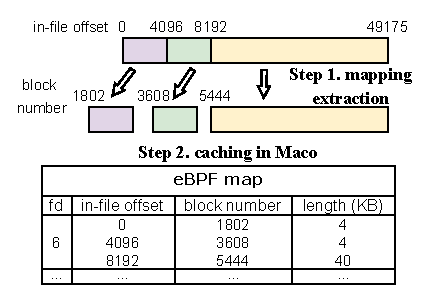
\includegraphics[width=0.9\linewidth]{fig/design/extractMap.pdf}
	%	\vspace{-1ex}
	\caption{An Illustration of \odes's Maco.}% Reorganizing Per-file Mappings}
\label{fig:prepare}
\vspace{-3ex}
\end{figure}

\subsection{ Donor-Based Online Space Allocation}\label{sec:design:donor}


%As mentioned, handling writes for a preallocated file is  more efficient than dealing with a growing one.
%However, to 
%In practice, using 
Using dynamically growing log files is also common for databases.
Let us enhance \odes
to serve databases  with such non-preallocated log files.
%use \odes's new path for growing files, we
%We must overcome a critical challenge:
%we need to consider several challenges
%That is,
%The stable structural layout of a preallocated file  eases the setup of per-file mappings to locate a target device block.
Note that a log file that expands over time demands that \odes
must track and keep the   changing per-file mappings, which is a non-trivial challenge for it. For example,
XRP~\cite{280870}, one prior study that attempts to optimize file read, manually updates the cached version of per-file mappings 
 every time some change has happened to a file's mappings. Note that
 this is feasible for file read, but infeasible for file write. % targeted by this paper.
%file write is a stark contrast to a file read. 
%The reason lies in updating the mappings.
For a file read, an update of per-file mappings % between   in-file offsets to  block numbers 
  has taken place
before the read request, hardly affecting the performance of   read operations.
%Therefore, the update does not significantly affect the performance of file read.
Nonetheless,
for a file write, the update itself is exactly part of the   write procedure and, worse, %more importantly,
occurs on the critical path with costly space allocation and file system journaling.
As mentioned in Section~\ref{sec:motivation}, 
%For example, %the data files of databases or scientific computing 
%given a file that gradually expands %in one or few blocks 
%due to appending writes, 
the   time  cost  per   write 
is  substantial for a growing file. % a preallocated file. 
%The latter two are costly actions as shown in Section~\ref{sec:motivation}.
%That is, ordinary file reads certainly occur after file writes, and the update of mapping will not be serious
 


To overcome this issue and enable \odes to take over non-preallocated log files,
%minimize the cost of updating per-file mappings and make \odes functional in handing appending writes for logging, 
we develop a preallocation-like strategy.
The core of this strategy is a    {\em donor pool}  of large files and the {\em move-extent} feature of Ext4~\cite{ext4moveextent}.
%that \odes prepares a pool of {\em donor files} with preallocated blocks. % in advance.  
 
%While preallocated files offer optimal performance, many production systems require dynamically growing log files. \odes introduces a novel donor-based allocation mechanism that achieves near-preallocated performance for growing files.

\textbf{Donor pool.} Initially,
\odes preallocates a pool of donor files. 
%These files would be utilized to resemble a preallocation effect at runtime.
Each donor file 
%\odes pre-reserves a pool of preallocated files as donors. A donor file 
is composed of a large contiguous space of blocks, initialized
%The contents of a donor file are all zeros.
%Each donor file is initialized
 by prefilling zeros.
To facilitate an efficient use of blocks in these donor files, \odes registers their per-file mappings  in the Maco structure in advance.

%The per-file mappings for them
%contiguous disk blocks organized as ``donor files.'' These donors are preallocated files with known, contiguous LBA ranges stored in Maco and persisted to disk. 



\textbf{Moving extents.} 
Ext4 originally uses \emph{move-extent} for online
defragmentation~\cite{ext4moveextent}. It exchanges extent mappings between two files without moving the mappings through the normal allocation path if both files do not have   valid data stored in exchanged extents.
\odes repurposes this interface for online space allocation.
For one such log file,
we intentionally  leave an unused block as a special tail, without holding any valid data.
%As to \
When a database intends to append data to unavailable space in the log file
and raises a request for space allocation,
%When the file is about to expand,
% instead of taking % triggering expensive runtime block allocation through 
%%%Ext4's conventional routine to initiate costly block allocations, 
%\odes leverages the {\em move\_extent} feature~\cite{ext4moveextent,mathur2007ext4}
%\odes uses the \texttt{EXT4\_IOC\_MOVE\_EXT} ioctl 
% \odes redirects the allocation to
% call \textit{move-extent} that swaps a range of blocks filled with zeros in a donor file
% with % (e.g., 1MB or 4MB) 
% the tail block of the  log file.
% %from a donor file to the target file.
% %\autoref{fig:des:move_extent} sketches how {\em move-extent} happens between two files. % a target file and a donor file.
\odes exchanges this tail block with a contiguous range from a donor file and updates the Maco mappings
accordingly. After the space exchange, the growing log file makes the last received block be the new tail.

%The \texttt{move\_extent} operation was originally designed for online defragmentation~\cite{ext4defrag}. 
%
\begin{figure}
	\centering
	\scalebox{0.75}{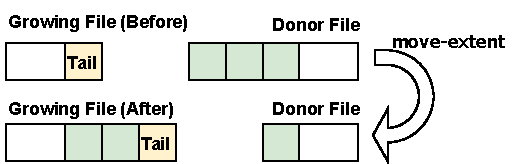
\includegraphics[width=\linewidth]{fig/design/move_extent.pdf}}
 %	\vspace{-1ex}
	\caption{An Illustration on how \odes uses the {\em move-extent} feature to expand a growing log file.}
	\label{fig:des:move_extent}
	\vspace{-3ex}
\end{figure}

\autoref{fig:des:move_extent} illustrates this process.
To reduce the frequency of space transfers and amortize the runtime cost of each \emph{move-extent} operation, \odes transfers a contiguous range that is larger than a typical logging write. Since logging I/O sizes may vary over time, \odes uses a lightweight monitor to track the moving average of recent write sizes and adjusts the transfer size accordingly. Based on our empirical study, \odes sets each transferred range to four times the observed average logging I/O size, providing sufficient space for several subsequent writes while avoiding excessive space reservation.

If the donor pool cannot satisfy an allocation request or a \emph{move-extent} operation fails, \odes falls back to Ext4's normal allocation path. Moreover, because \odes prepares extents asynchronously
through io\_uring, a write may arrive before the corresponding
\emph{move-extent} completes. In this case, the write waits for completion
before using the new mapping, preventing it from observing a partially
updated mapping.
\begin{comment}
  % \autoref{fig:des:move_extent} briefly illustrates how \odes leverages the move-extent feature, and
% this donor-based strategy enables an efficient on-the-fly preallocation. 
\autoref{fig:des:move_extent} illustrates this process.
% high efficiency and performance. % several critical advantages:
First, as  donor files are  preallocated and registered in the Maco structure,  \odes    quickly transfers
blocks to the target log file
and  updates the Maco for both files. %, without querying the extent trees for both.
Second, \odes moves  a contiguous  range of blocks at a time to minimize the runtime cost.
%The target file may expand for a long stretch, or just one to few blocks at one time. 
In light of our observations (see Section~\ref{sec:motivation}), the allocation space shall be  greater
than the typical size of  logging I/Os. We calculate a moving average of write requests online over a time window  by a simple  monitor module
%The measurement of I/O requests can be done by a simple online monitor,
and   empirically set the transferred space  four times of the average logging I/O size.
%This batched allocation   incurs minimal journaling overhead.
%By doing so, the journaling overhead is likely to be minimized.
%Whereas, \odes insists on transferring a range of blocks (e.g., 128 KB or 1 MB).
%so that the journaling overhead due to changing the metadata for both files shall be amortized.
% The accumulated cost of triggering the journaling for multiple times is much more than that of doing in a joint batch.
When the log file is closed, \odes transfers back  blocks that are not used to the source donor file, in order to avoid % thereby avoiding
 space waste in the donor pool.

\odes sets the size of the transferred space from the logging I/O sizes that the
monitor module measures, replenishes the donor pool in the background, and reclaims
unused blocks when a log file is closed. As described
above, \odes decides online how much space to transfer at a time 
%, by setting the transferred space to four times the average logging I/O size that the monitormodule measures over a time window, 
and returns the unused blocks when the log file is closed. Once
the free space of the donor pool drops below a threshold, \odes preallocates new
donor files to replenish the donor pool off the critical path. If the donor pool
cannot satisfy a request for space, or if a move-extent operation fails, \odes
falls back to Ext4's normal allocation path for the request. The log file remains
correct, because the correctness of a logging write never depends on the donor
pool, and the request loses only the acceleration that \odes would otherwise
provide. Since \odes issues move-extent operations ahead of time through io\_uring, a
write request may arrive before the move-extent operation that prepares space for
the write request has completed; in such a case \odes lets the write request wait
until the move-extent operation completes, so the write request never observes a
partially updated mapping.
\end{comment}


%%in order to avoid space waste in the donor pool.
% the preallocation of donor files helps to obtain 





\begin{comment}
to regulate the use of donor files and match different usage patterns of 
applications, we include an exponential-step mode
for transferring donor's blocks. In short, 
for files that do not aggressively ask for blocks, we transfer a range of blocks, e.g., 128 KB at a time.
But for a target file that demands some blocks for the first time but soon 
launches the next request,
%demands furthermore space soon, 
we transfer doubled space, i.e., 256 KB. 
We continue to transfer, 512 KB, 1 MB, and so on until a predefined limit. 
In practice, we set this limit to be 128 MB, which is the maximum extent size supported by Ext4 \cite{Ext4:extent-size}.
%enables \odes 
%to support dynamically growing files
 % with performance approaching that of preallocated files, 
%while maintaining full compatibility 
%with existing database systems that rely on dynamic allocation.
\end{comment}


\begin{comment}
 

\begin{itemize}
\item Since donor blocks have predetermined addresses, \odes can immediately update Maco without querying Ext4's extent tree.

\item \textbf{Contiguous layout:} Donor pools ensure that growing files receive contiguous blocks, maintaining sequential I/O performance.
\end{itemize}

\textbf{Growth Strategies for Journal Optimization.}
To minimize journaling overhead from repeated inode modifications, \odes offers two configurable growth strategies:

\textit{1. Maximum-size mode:} On the first append operation, the file is immediately extended to a predetermined maximum size (e.g., 4MB for a 4KB file). This incurs journal overhead only once, with all subsequent writes operating within the pre-extended space. This mode is ideal for files with predictable growth patterns.

\textit{2. Exponential-step mode:} Files grow in exponentially increasing steps: 1MB, 2MB, 4MB, up to 512MB. Each step incurs a single journal write, but the exponential growth ensures that the number of journal operations remains logarithmic in file size. When a file is closed, unused donor blocks are returned to the pool, preventing storage waste.


\begin{algorithm}
\caption{Donor-Based File Extension}
\label{alg:donor}
\begin{algorithmic}[1]
\STATE \textbf{procedure} ExtendFile($file$, $size\_needed$)
\STATE $current\_size \gets$ GetFileSize($file$)
\STATE $target\_size \gets$ DetermineTargetSize($current\_size$, $size\_needed$)
\STATE $blocks\_needed \gets$ $(target\_size - current\_size) / block\_size$
\STATE 
\STATE $donor \gets$ SelectDonorWithBlocks($blocks\_needed$)
\IF{$donor = null$}
    \STATE \textbf{return} FallbackToNormalAllocation()
\ENDIF
\STATE
\STATE $donor\_extent \gets$ GetContiguousExtent($donor$, $blocks\_needed$)
\STATE $result \gets$ ioctl($EXT4\_IOC\_MOVE\_EXT$, $file$, $donor$, $donor\_extent$)
\STATE 
\IF{$result = success$}
    \STATE UpdateMaco($file$, $donor\_extent.lba\_start$, $blocks\_needed$)
    \STATE MarkDonorBlocksUsed($donor$, $donor\_extent$)
\ELSE
    \STATE \textbf{return} FallbackToNormalAllocation()
\ENDIF
\STATE \textbf{return} $success$
\end{algorithmic}
\end{algorithm}
\end{comment}

\begin{comment}
 

\subsection{Security-Aware Dual-Mode Architecture}\label{sec:design:security}

A fundamental challenge for any kernel-bypass solution is maintaining security while optimizing performance. \odes addresses this through a dual-mode architecture that decouples the high-performance data path from the kernel's trusted security enforcement, respecting both Linux security models (DAC and MAC) introduced in Section \ref{sec:background}.

\textbf{Security Initialization via \texttt{open()} Syscall.}
\odes intentionally preserves the standard \texttt{open()} syscall path as a critical security handshake. When a database opens a log file, the kernel performs standard permission validation:
(1) DAC checks validate user/group/other permissions against the file's mode bits, and
(2) MAC frameworks (SELinux, AppArmor) enforce system-wide policies through LSM hooks.
Only after successful validation does \odes extract metadata, ensuring it operates exclusively on legitimately accessed files.

\textbf{Fast Mode: DAC-Aligned Performance Optimization.}
The default Fast Mode aligns with DAC's check-on-open semantics. Since DAC validates permissions only during \texttt{open()}, subsequent I/Os through the file descriptor proceed without rechecking. \odes leverages this characteristic by:
\begin{itemize}
\item Relying on the initial \texttt{open()} validation for security
\item Bypassing per-I/O permission checks entirely
\item Directly dispatching I/Os to device drivers via cached LBA mappings
\end{itemize}
This mode is safe for database logging where permission changes during runtime are exceedingly rare—databases open their own log files with write permissions that remain stable throughout execution.

\textbf{Strict Mode: MAC-Compliant Per-I/O Validation.}
For environments requiring continuous security validation (typical in MAC-enforced systems), Strict Mode ensures permission checks on every I/O operation. Unlike the full kernel path, \odes achieves this efficiently:
\begin{itemize}
\item eBPF hooks intercept each write/fdatasync operation
\item Lightweight kernel helpers validate permissions without full stack traversal
\item Both inode attribute and LSM policies are checked per-I/O
\item Failed checks immediately return \texttt{EPERM} or \texttt{EACCES} errors
\end{itemize}

\begin{algorithm}[t]
\small
\caption{Security-Aware I/O Interception}
\label{alg:permission}
\begin{algorithmic}[1]
\STATE \textbf{procedure} InterceptWrite($fd$, $buffer$, $size$)
\STATE $file \gets$ GetFileFromFD($fd$)
\STATE $mode \gets$ GetSecurityMode() \COMMENT{Fast or Strict}
\IF{$mode = FAST$}
    \STATE \COMMENT{Trust initial open() validation—no recheck}
\ELSIF{$mode = STRICT$}
    \STATE Validate DAC permissions via eBPF helper
    \IF{DAC check fails} 
        \STATE \RETURN $EPERM$ 
    \ENDIF
    \IF{LSM active}
        \STATE Validate MAC policies via eBPF helper
        \IF{MAC check fails} 
            \STATE \RETURN $EACCES$ 
        \ENDIF
    \ENDIF
\ENDIF
\end{algorithmic}
\end{algorithm}

This dual-mode design allows administrators to choose between maximum performance (Fast Mode for DAC-only environments) and strict security compliance (Strict Mode for MAC-enforced systems), ensuring \odes adapts to diverse deployment requirements while maintaining security integrity.

\subsection{Forward Compatibility}
\odes is functional with both SATA and NVMe SSDs. For SATA SSD, \odes uses the SCSI abstraction layer rather than sending ATA commands directly~\cite{T10Techn64:online}, because many Linux distributions restrict direct ATA transmission~\cite{libATADe51:online}. Yet passing I/Os via the SCSI layer introduces negligible overhead relative to overall I/O latency. This guarantees that \odes remains compatible and usable with a wide range of storage devices.
\end{comment}


\subsection{Optimizations and Discussions}\label{sec:design:discussion}
{\bf Optimizations.}
%Using the donor-based strategy, \odes retains the   preallocation-like 
%Now \odes retains the preallocation-like 
%advantage in processing   writes for both preallocated and   growing log files.
We   optimize \odes with two tactics.
%One is for scalability.
First, %we %do not synchronously calling the {\it move-extent} to exchange extents,
%for extension
%but 
we leverage the   io\_uring~\cite{iouring,ioctlWik84:online} to asynchronously transfer extents for non-preallocated log files. %transfers.
%do so asynchronously with the io\_uring \cite{iouring,ioctlWik84:online}. 
The io\_uring provides user-space asynchronous I/O interfaces, %~\cite{iouring,ioctlWik84:online}.
while
the eBPF used by \odes 
sits at the boundary between kernel and user spaces.
%Hence,
As a result,
%At runtime,
while dealing with an ongoing   write at runtime,
%When handling a write request, 
\odes  simultaneously executes the {\it move-extent} through io\_uring to prepare for future writes.
%in the meantime, 
In brief, it parallelizes handling
%thereby parallelizing 
the current logging write with demanding space for   incoming ones.
%while the eBPF used by \odes
This overlapped execution    reduces the cost of invoking   {\it move-extent}
on the critical path.
Second, for high scalability
we partition  the  Maco and donor pool, and distribute them to be per-core  structures. 
In other words, we make them decentralized to reduce contention issues.
%thereby making them
%and make them 
%decentralized  for high .scalability


% {\bf Crash consistency.} \odes changes where a logging write is delivered, but
% changes neither the content of the write nor the moment at which the write is
% declared persistent. \odes writes the same bytes to the same device blocks, because the
% block numbers that \odes uses come from Ext4's own extent tree. For ordering, \odes
% synchronously waits for the return signals of write and fdatasync before returning
% to the database, so the order on which a database relies, i.e., completing the
% logging write ahead of the in-place update of database records, stays unchanged.
% For persistence, an SSD with PLP quickly completes a flush, and if an SSD does not
% have PLP, \odes explicitly issues a flush command, such as the {\tt nvme-flush} of
% NVMe protocol, to drain the SSD's internal cache, so that the shortcut I/O path
% provides the same persistence semantics as the original
% fdatasync~\cite{fsync:bio-flags}. 
% For a partial write, \odes returns the same
% error to the database as the conventional path returns when the device reports a
% write as failed or incomplete. Databases already protect log records with
% checksums and, at recovery, recognize and discard an incomplete record at the tail
% of the log file, exactly as databases do after a crash on the conventional path.
% For metadata after a crash, the Maco structure holds no state that Ext4 cannot
% derive on its own: \odes builds the Maco structure from the extent tree when
% opening the log file, and for a growing log file the only operation that changes
% the Maco structure is the move-extent that \odes itself issues. Move-extent is an
% operation of Ext4, and Ext4 journals every move-extent. Ext4's on-disk metadata is
% therefore authoritative after a crash, and \odes rebuilds the Maco structure when
% the log file is opened next time, so a crash leaves behind no mapping that only
% \odes knows. \odes writes data into transferred space only after the corresponding
% move-extent has completed, so the case never arises that data has already been
% written into blocks while Ext4 still regards the blocks as belonging to the donor
% file. If a move-extent operation fails, or if the donor pool cannot satisfy a
% request for space, \odes falls back to Ext4's normal allocation path.

% 0823 zl: Do 'so the order on which a database relies, i.e., completing the logging write ahead of the in-place update of database records, stays unchanged.' need to be kept? 

{\bf Crash consistency.} \odes preserves crash consistency by changing only the I/O path, while maintaining the write ordering and persistence semantics expected by the database. It writes to device blocks obtained from Ext4's extent tree and synchronously waits for write and `fdatasync` completion before returning. %, so the order on which a database relies, i.e., completing the logging write ahead of the in-place update of database records, stays unchanged.
For persistence, \odes relies on device power-loss protection (PLP) when available; otherwise, it explicitly issues a device flush, e.g., an {\tt nvme-flush}, to drain volatile caches~\cite{fsync:bio-flags}.

\odes also preserves conventional partial-write behavior. If a write completes only partially, it returns the corresponding error, allowing the database's existing checksum and recovery mechanisms to detect and discard incomplete log records.

Finally, \odes introduces no independently persistent mapping metadata. The Maco structure is reconstructed from Ext4's extent tree when the log file is opened, and runtime mapping changes occur only through journaled move-extent operations. \odes writes to transferred space only after move-extent completes, ensuring that Ext4's metadata is updated before the new blocks are used. If move-extent fails or the donor pool lacks sufficient space, \odes falls back to Ext4's normal allocation path.


% {\bf Stale mappings.} The per-file mappings that \odes caches in the Maco structure
% do not become stale during the period in which \odes uses the mappings. For a
% preallocated log file, writing data into already allocated space triggers no block
% allocation, and a database neither truncates nor reallocates a log file that the
% database is appending data to, so the mappings of a preallocated log file do not
% change while the log file stays open. For a growing log file, the only operation
% that changes the mappings is the move-extent that \odes itself issues, and \odes
% updates the Maco structure in the same step. \odes builds the Maco structure when
% opening the log file and discards the Maco structure when closing the log file, so
% the Maco structure exists exactly during the period in which the log file stays
% open. An operation that happens while the log file is not open, for example Ext4's
% online defragmentation, therefore leaves no outdated entry in the Maco structure. In the strict mode, moreover, \odes verifies inode
% attributes through ioctl interfaces at every operation, and such verification also
% observes a change of file metadata.

{\bf Stale mappings.}  \odes keeps cached mappings only while a log file is open. For a preallocated log file, appending to already allocated space does not change its block mappings. For a growing log file, mappings change only through move-extent operations issued by \odes, which update the Maco structure accordingly. When the file is closed, \odes discards the Maco structure and rebuilds it from the file-system metadata upon the next open, preventing changes between opens from leaving stale cached mappings. In strict mode, \odes additionally re-validates permission through a kernel-space LSM check at every operation, and such verification also observes any change of file metadata.

{\bf Error reporting.} The ioctl interfaces return the completion status of the
device to \odes, and \odes maps the completion status onto the same errno that the
conventional path returns on write or fdatasync. A database therefore sees the same
errors as the conventional path returns, and the error handling logic that the
database already has needs no change.

{\bf Permission checks.} 
 Linux has two models for     permission checks, i.e., the Discretionary
Access Control (DAC) and Mandatory Access Control (MAC). 
DAC checks   permission   at
opening a file. MAC does so at each file operation.
%There are two main permission checks for file operations. 
%We have talked about two level permissions in the 
%Note that databases 
Databases hardly change the access permission of log files, e.g., from read/write to read-only.
%a runtime change of  access permission for a database log, say, from read/write to read-only, is very rare. 
Though, we
%This operational characteristic enables \odes' dual-mode architecture. 
make  configurable dual modes for \odes.
Its {\em fast mode} aligns  with DAC's one-time validation for   performance.
% is for optimal performance by aligning with DAC's one-time validation. 
%For enhanced protection, the 
The {\em strict mode} follows  MAC compliance for enhanced protection
 through   a lightweight kernel-space permission check at the LSM hook of every    operation.
% to ensure comprehensive integrity validation.

{\bf Compatibility.}
\odes   is  functional with both SATA and NVMe SSDs. This is a contrast to prior designs like BypassD working for NVMe SSDs only.
For SATA SSD, \odes uses the SCSI abstraction layer rather than sending ATA commands directly, % \cite{T10Techn64:online},
 because many Linux distributions restrict direct ATA transmission \cite{libATADe51:online}. 

%  08.23 zl: remove
% {\bf Portability.} Some parts of \odes are general, while other parts depend on a
% specific file system, operating system, or device. Caching the per-file
% offset-to-block mappings and consulting the cached mappings at runtime only require
% that the mappings of a file stay stable while the file is open, and any file system
% that allocates blocks and updates data in place, including Ext4 and XFS, meets the
% requirement. The donor-based online space allocation additionally requires that
% the file system provide an interface that exchanges a range of space between two
% files without copying data. Ext4 provides move-extent~\cite{ext4moveextent}, and
% XFS provides a range-exchange ioctl that serves the same
% purpose~\cite{xfs-exchange-range}. On file systems that write data out of place
% instead of updating data in place, such as Btrfs and F2FS, every overwrite changes
% the mappings of a file, so the requirement of stable mappings does not hold and
% \odes would need another way to obtain block numbers. Intercepting syscalls with eBPF and
% delivering data through ioctl interfaces are both specific to Linux. The flush command
% is specific to the device, and \odes already issues the commands of both NVMe and
% SCSI.

{\bf Portability.} \odes is readily portable to Linux systems using in-place-update file systems, such as Ext4 and XFS, on NVMe or SCSI devices. Its portability mainly depends on three components. First, the cached offset-to-block mappings require file block mappings to remain stable while a file is open, which is naturally supported by in-place-update file systems. Out-of-place-update file systems, such as Btrfs and F2FS, require additional mechanisms to track block mappings because overwrites may change the underlying block locations. Second, donor-based online space allocation requires a file-system interface for exchanging storage ranges between files without data copying, such as Ext4 move-extent~\cite{ext4moveextent} and XFS range-exchange~\cite{xfs-exchange-range}. Third, syscall interception and data delivery rely on Linux eBPF and ioctl interfaces, while device flushing requires device-specific commands, for which \odes currently supports both NVMe and SCSI. 

%Passing I/Os via the SCSI layer introduces negligible overhead relative to overall I/O latency, but   guarantees that \odes remains compatible and usable with a wide range of storage devices. 


\begin{comment}
 
\subsection{Discussions}\label{sec:design:discussion}

\textbf{Applicability.}
\odes builds a shortcut write path from   application to device driver, without involving the OS's page cache.
Therefore, it is not only fit for applications that cache data in their user-space buffers, 
%such as databases,
but also useful for applications that save intermediate or eventual results for subsequent use.
  For example, 
databases prefer to manage data on their own, by caching data in user-space caches  
%,
%rather than the OS's page cache, 
%to accelerate search operations.
to satisfy search requests
and writing data to a log before in-place update for crash recovery. 
 As
logging is a time-consuming operation that impairs the performance of databases,
\odes is helpful to reduce the cost of logging  for them.
%hey can reduce the time cost of logging through the utilization of \odes.
%As logging is time-consuming, databases will benefit from the utilization of \odes.
Moreover,
large-scale deep neural networks, such as the large language models (LLM),
generally require  a long time for training. Thus, checkpointing a model's states and parameters into persistent storage
in the middle of training
helps to quickly restore the training process in case of an unexpected failure \cite{264850,10630969}.
Many scientific computing 
applications often produce a large amount of results in an experiment.
They accumulate those results
%for persistent store
 and conduct analytical investigation later.
\odes shall be   effective in these circumstances too. 
%Moreover,
%Furthermore,

%\odes shall be well functional in these circumstances.


%TODO: this part should be refined with huyp -- wangc@2025.09.10-08:46am
\textbf{Access control.} By default, Linux applies the DAC for one-time check of access permission %(e.g., read-only or write/read) 
at opening a file. 
This is generally used in real-world practices.
Whereas, there are applications requiring continuous security validation. % (typically in MAC-enforced systems),
We enhance \odes to support the MAC-enforced  permission check
%Strict Mode ensures permission checks 
on every I/O operation. 
To implement
%\odes achieve 
this stricter mode,
we mainly utilize the   LSM (Linux Security Modules) hooks \cite{270581,kernel-LSM,eBPF-LSM}.
%Unlike the conventional path, 
%It . 
%The eBPF LSM mechanism 
The classic LSM framework was developed more than two decades ago
to enable general
support for access control in   Linux kernel \cite{270581,kernel-LSM}. 
LSM
mediates an access to kernel objects (e.g., files) for permission check \cite{270581} by
placing  hooks  (function calls) at critical points in the kernel code, right before a concerned action (e.g., file write or fdatasync)
% emphasized in this paper) 
is about to happen.
%and 
%In short,
%it is used to 
Since Linux kernel  5.7, %%% released in 2020, 
the eBPF LSM has been introduced \cite{eBPF-LSM,prog-LSM}, which makes \odes achieve  the
MAC effect efficiently on the fly. %%% by inspecting a file write or fdatasync syscall.
%which helps \odes flexibly achieve MAC .
To this end,
 the eBPF LSM hooks intercept  each file write and fdatasync, and \odes has 
a  kernel-space  helper to check the file's inode attributes for verification.
Only after a successful validation does \odes query the Maco % metadata
and continue on its path, ensuring that it operates   with a legitimately accessed file.
%A pass will continue alongside the I/O path of \odes, while
A failed check immediately returns with an  \texttt{EPERM} or \texttt{EACCES} error.

\end{comment}



\begin{comment}
\begin{itemize}
	\item eBPF hooks intercept each write/fdatasync operation
	\item Lightweight kernel helpers validate permissions without full stack traversal
	\item Both inode attribute and LSM policies are checked per-I/O
	\item Failed checks immediately return \texttt{EPERM} or \texttt{EACCES} errors
\end{itemize}
\end{comment}

%\textbf{Truncation.} \todo{how to do?}



\begin{comment}
 

\subsection{Putting Everything Together for \odes}\label{sec:design:summary}
\odes is a comprehensive solution for eliminating software tax on database logging writes. % with three key innovations.
Firstly, 
%\textbf{1. Intelligent Path Optimization.} 
by intercepting file operations with the eBPF and redirecting them via ioctl interfaces, \odes bypasses 
almost all kernel layers of the stock storage stack.
%It makes use of device-specific commands, such as \texttt{nvme-flush}, % for NVMe SSD, 
%for acceleration.
%five of the six traditional I/O layers (VFS, filesystem, journaling, block layer, and scheduler), 
%reducing software overhead by up to 62.9\%. 
%The system maintains correctness through explicit cache flushes (e.g., \texttt{nvme-flush}) to ensure durability semantics.
Secondly,
\odes seamlessly supports both preallocated and   growing log files. 
For preallocated ones, it extracts and reorganizes per-file mappings at initialization. For growing files, the donor-based preallocation-like strategy pre-reserves contiguous spaces and exploits Ext4's \textit{move-extent} feature
to extend files in minimal cost, achieving the effect of preallocation without sacrificing flexibility.
%Last but the not least, \odes provides two modes for access control,
%such that security-critical environments can maintain per-request validation 
%without losing the performance boost that \odes's fast   path enables.

\end{comment}
%\textbf{3. Flexible Security Preservation.} The dual-mode architecture allows administrators to choose between maximum performance (Fast Mode) and strict security compliance (Strict Mode). This design recognizes that database log files have stable permission patterns while ensuring that security-critical environments can maintain per-I/O validation without sacrificing the benefits of the optimized I/O path.

%Through this integrated design, \odes achieves up to 2.3× throughput improvement for write-intensive workloads while maintaining full POSIX compatibility, requiring no application modifications, and supporting both SATA and NVMe storage devices.

